\chapter{Conceptos previos} 
\label{chap:conceptos previos}
Este capítulo trata de recoger y exponer los principales conceptos y tecnologías implicadas en los despliegues en los que se usa Openstack.

Para ello iremos desde el concepto de virtualización hasta llegar al cloud computing, pasando por la tecnología de contenedores a la par que analizamos los beneficios de estos y algunos inconvenientes para acabar hablando de la virtualización de funciones de red o NFV y el rol que OpenStack tiene en ella.

\section{De la virtualización al Cloud Computing}

A lo largo de los años, la informática corporativa ha visto muchos desarrollos que han derivado en el aumento de la computación en la nube tal como la conocemos:

\begin{itemize}
\item En la década de 1990, la informática corporativa se centraba en servidores en un centro de datos.
\item En la década de 2000, la informática corporativa se basaba principalmente en la virtualización.
\item En la década de 2010, estamos viendo el aumento de la computación en la nube para aprovechar la informática corporativa.
\end{itemize}

\subsection{Virtualización}
Para introducir los contenidos que trataremos, vamos a hablar en primer lugar de qué es la virtualización. Cuando se habla de virtualización, la mayoría de las personas piensa en máquinas virtuales. Una máquina virtual \textit{(Virtual Machine, VM)} es una computadora en la que el software, así como el hardware, se crean como una solución de software que simula un sistema de computación  y puede ejecutar programas como si fuese una computadora real. El objetivo de la virtualización es proporcionar una versión virtual, en lugar de física, de los activos de TI esenciales:

\jorge{RECOMENDACIÓN: Usa dos apóstrofes en vez de comillas, porque en LaTeX da menos problemas (depende de dónde escribas las comillas generan errores). Y se usa itemize para meter dentro todos los items, no pongas un itemize para cada item. Te comento esto por los errores que pueda darte. Si no hay errores y quieres dejarlo como está, perfecto.}

\begin{itemize}
\item 
\textbf{Hardware}: Este es el uso ''tradicional'', donde el sistema operativo se instala en una representación de software de los recursos de hardware.
\item 
\textbf{Almacenamiento}: También conocido como almacenamiento definido por software (\textit{Software Defined Storage, SDS}). En SDS, se crea una capa entre los discos duros reales y las computadoras que acceden a estos discos duros, con el 	objetivo de hacerlos más accesibles.
\item 
\textbf{Redes}:	Las actuales redes definidas por software (\textit{Software Defined Networks, SDN}). En SDN, los usuarios de la nube pueden crear una infraestructura de red lógica en la parte superior de la red física, lo que hace que sea más fácil satisfacer sus necesidades.
\end{itemize}


\subsection{Beneficios de la virtualización}
En OpenStack, se utilizan todos los tipos de virtualización. La virtualización tiene muchos beneficios para las IT modernas:

\begin{itemize}
\item 
Permite un uso más eficiente de la capacidad del servidor físico. Si se observa la utilización típica de la CPU de los servidores de hardware, lo más probable es que veamos una utilización de CPU inferior al 10 o incluso al 5\%. La virtualización permite ejecutar diferentes máquinas virtuales sobre CPUs físicas, lo que significa que el uso de la CPU se puede optimizar para colocarnos en torno al 80\%.
\end{itemize}

\begin{itemize}
\item 
Permite un uso más eficiente del espacio físico destinado al centro de datos. Este es un gran problema porque el espacio del centro de datos es caro. Imaginemos que deseamos construir un centro de datos en el medio de una gran ciudad. Los metros cuadrados en las grandes ciudades en general son muy caros. Y esa es la razón por la cual la virtualización ayuda en este sentido, porque el uso de máquinas virtuales significa que necesitaremos menos hardware físico, y usar menos hardware físico significa usar menos metros cuadrados con el consecuente ahorro económico. 
\end{itemize}

\begin{itemize}
\item 
Permite un consumo de energía más eficiente. Como resultado de lo anterior, también podremos usar la energía de una manera más eficiente, si pensamos en las facturas de electricidad de los centros de datos corporativos grandes, que pueden llegar a millones. Por tanto, si optimizamos los servidores reduciendo a la mitad la cantidad de servidores físicos que se necesitan, mejoraremos en esto aspecto, utilizando así la mitad de la energía necesaria para ejecutar estos servidores, lo que permite a las compañías ahorrar una gran suma.
\end{itemize}


\subsection{Implicaciones de la Virtualización}
Cuando se trata de virtualización, los activos físicos están representados por software:
\begin{itemize}
\item 
Los servidores y las estaciones de trabajo se están convirtiendo en máquinas virtuales.
\end{itemize}
\begin{itemize}
\item 
Las redes y el almacenamiento también se pueden virtualizar, convirtiéndose así en SDN y SDS.
\end{itemize}
\begin{itemize}
\item 
Con todos estos tipos de virtualización, un administrador puede construir un \textit{data center} definido por software.
\end{itemize}

\subsection{Limitaciones de la virtualización}
Aún así, la virtualización también tiene algunas limitaciones:
\begin{itemize}
\item 
La ausencia de soluciones de autoservicio. En virtualización, es el administrador quien proporciona la infraestructura que está creando el almacenamiento, la red y las máquinas virtuales. Como usuario final, solo se podrá solicitar la virtualización de los recursos para a continuación esperar a que el administrador tenga tiempo para cumplir con esta solicitud.
\end{itemize}
\begin{itemize}
\item 
Escalabilidad limitada. Por supuesto, hay escalabilidad, porque se pueden agregar servidores a la virtualización para alojar más máquinas virtuales, y también se pueden agregar redes, así como almacenamiento. Pero el hecho de que sea el administrador el encargado de estas tareas, hace que la escalabilidad se encuentre restringida. 
\end{itemize}
\begin{itemize}
\item 
La virtualización es relativamente pesada, ya que cada VM tiene su propio kernel. Si estamos ejecutando veinte máquinas virtuales en un \textit{host} de hipervisor, estamos ejecutando veinte kernels diferentes. Si se necesitan, sin embargo, máquinas virtuales con diferentes sistemas operativos, no hay realmente otra solución para hacerlo de manera más eficiente. Por el contrario, si estamos ejecutando sistemas operativos similares, podemos hacerlo de manera más eficiente, y ese es exactamente el objeto de la tecnología de contenedores.
\end{itemize}

\jorge{¿Qué quieres decir con ''un host de hipervisor''? ¿Sería ''un host que actúa como hipervisor''?}

\subsection{Virtualización basada en host vs basada en hipervisor}

La solución más común utilizada para ejecutar máquinas virtuales sobre Linux en un centro de datos es KVM \textit{ (Kernel-based Virtual Machine)}. KVM es un tipo de virtualización basada en hipervisor (como es el caso de otras soluciones como \textit{VMware ESXi}). Cuando se trata de  virtualización basada en hipervisor, la máquina virtual se ejecuta sobre un kernel de virtualización pequeño y altamente optimizado, que permite a la máquina virtual abordar el hardware de manera más eficiente tal como se esquematiza en la parte izquierda de la Fig.\ref{Container vs VM}.

Otra solución de virtualización común es \textit{VirtualBox} (basada en \textit{host}). VirtualBox permite a los desarrolladores ejecutar un sistema operativo virtual en la parte superior de su escritorio. Sin embargo, esta solución no es tan eficiente como la virtualización basada en hipervisor.

\jorge{Yo pondría una descripción un poco más técnica del caso de virtualización basada en host. Entiendo que te refieres a que se utiliza un kernel de propósito general, como el que se encuentra en las distribuciones de Linux, y por tanto no está tan optimizado...}

En el caso de la infraestructura como servicio, las soluciones actuales utilizan virtualización basada en hipervisor.

\subsection{Tecnología de contenedores}
Como solución al problema del peso de la virtualización, surgió la tecnología de contenedores. En IT, el objetivo fundamental es ejecutar una aplicación, y no una máquina virtual. Al fin y al cabo, es el usuario de la aplicación quien tiene una necesidad. Esta necesidad es ejecutar una aplicación, y ningún usuario pedirá, por lo general, una máquina virtual (aunque actualmente existen empresas que están desplegando precisamente este tipo de servicios). Ese es, pues, uno de los principales objetivos de diseño de la tecnología de contenedores.

\begin{figure}
    \centering
    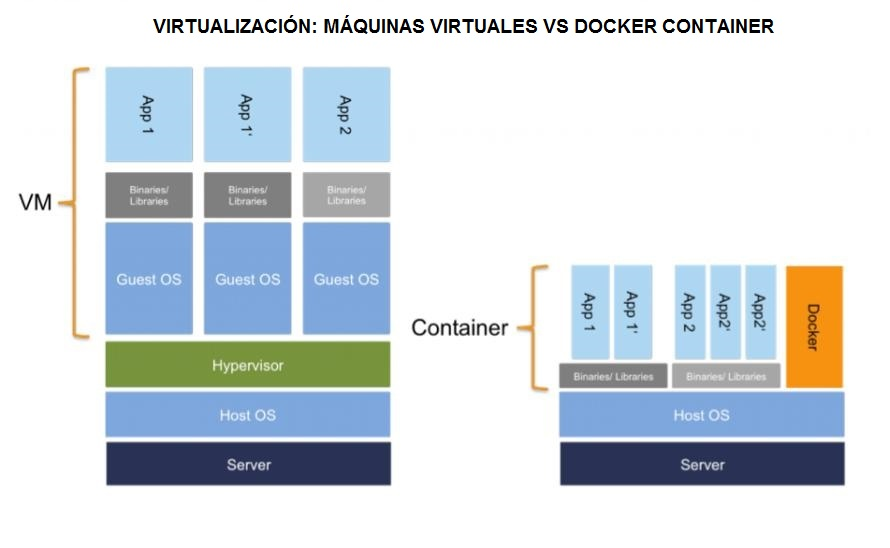
\includegraphics[width=1\textwidth]{imagenes/capitulo1/docker-vm-container.png}
    \caption{Containers vs VMs.}
	\vspace{0.3cm}
    \footnotesize{Fuente: Crisp Research, “Container-Technologien auf dem Vormarsch: Docker in a Nutshell”, 2014}
    \label{Container vs VM}
\end{figure}

Un contenedor es un método de virtualización en el nivel del sistema operativo. Esto permite que varias instancias de un sistema operativo se ejecuten en el mismo kernel, lo que permite un uso más eficiente de los recursos disponibles.

Usar contenedores  facilita a los usuarios finales ejecutar aplicaciones en diferentes plataformas. Las tecnologías de contenedores, como \textit{Docker}, eliminan la necesidad de considerar las diferentes características de la plataforma. El contenedor simplemente se ejecuta como un entorno aislado en la parte superior de la plataforma. Todo lo específico de la aplicación se incluye en un paquete que se ejecuta en la parte superior de cualquier plataforma de hardware. Esto permite al desarrollador centrarse en la aplicación, no en la plataforma subyacente.

Por  tanto, el desafío dentro de un entorno de IT moderno típico es el hecho de la existencia de una gran cantidad de entornos de hardware y multitud de stacks o pilas que necesitan soporte. Cuando hablamos de una pila  o stack, estamos hablando de un entorno completo que se usa para abrir los contenedores, como se puede ver a la derecha de la Fig. \ref{Container vs VM} en comparación de la pila usada para las máquinas virtuales que vemos en la izquierda. 

\begin{figure}
    \centering
    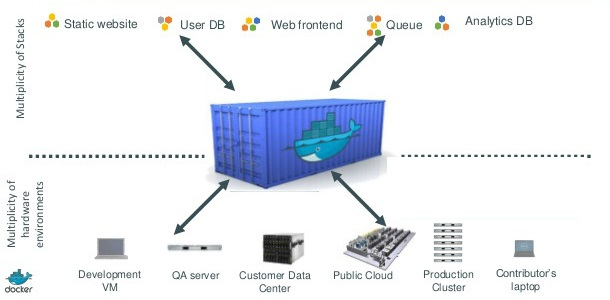
\includegraphics[width=1\textwidth]{imagenes/capitulo1/docker-stacks.png}
    \caption{Docker stacks.}
	\vspace{0.3cm}
    \footnotesize{Fuente: Docker }
    \label{Docker stacks}
\end{figure}

Algunas pilas existentes se ilustran en la Fig.\ref{Docker stacks}, como un sitio web estático, una base de datos de usuario (\textit{user DB}), una interfaz web, una cola o una base de datos de análisis \textit{(analytics BD}). Estas pilas son más que sólo la aplicación, hay un entorno completo que se necesita para ejecutar la pila en la parte superior de un sistema operativo. El propósito de la contenerización es ponerlo todo en un contenedor, de forma que creamos un paquete autónomo donde todo está incluido con el fin de poder ser manipulado usando operaciones estándar y ejecutarse consistentemente en prácticamente cualquier plataforma de hardware como puede ser una VM, un servidor de QA (\textit{Quality Assurance}), un centro de datos de clientes, una nube pública, un \textit{cluster} de producción, una PC portátil, etc.

Por lo tanto, al trabajar con contenedores, los desarrolladores de aplicaciones pueden eliminar los problemas relacionados con la ejecución de aplicaciones sobre diferentes sistemas operativos.

De esta forma, en general, la tecnología de contenedores está haciendo que las IT sean más eficientes.

\begin{itemize}
\item Se pueden implementar fácilmente muchas instancias de una aplicación para que se ejecute sobre un kernel único.
\item Este kernel proporciona entornos aislados y, por lo tanto, seguros.
\item A su vez, esto hace que los contenedores en ejecución sean un proceso seguro: un usuario de un contenedor no puede acceder a los recursos que están asignados a otro contenedor. 
\item Debido al hecho de que muchos contenedores se pueden usar sobre el mismo kernel, los recursos se pueden usar de una manera más eficiente. 
\item La implementación es mucho más llevadera debido al tamaño relativamente pequeño de los contenedores.
\end{itemize}

¿Cuáles son por tanto las diferencias entre los contenedores y la virtualización? Básicamente que los contenedores y la virtualización se utilizan en diferentes contextos:

\begin{itemize}
\item Usaremos contenedores si queremos ejecutar múltiples copias de una sola aplicación, con lo que podremos balancear la carga. 
\item Por otro lado, usaremos máquinas virtuales si necesitamos la flexibilidad de ejecutar múltiples aplicaciones o si queremos poder ejecutarlas en cualquier sistema operativo.
\end{itemize}

Tanto los contenedores como las máquinas virtuales se pueden ejecutar juntos en una nube IaaS.

\section{Cloud Computing}
La computación en la nube o \textit{Cloud Computing}, es un tipo de computación basada en Internet que proporciona recursos de procesamiento compartido y datos a computadoras y otros dispositivos bajo demanda. Permite el acceso bajo demanda a un grupo compartido de recursos informáticos, como redes, servidores, almacenamiento, aplicaciones y servicios, que normalmente están alojados en centros de datos de terceros. La computación en la nube es una metáfora para hacer referencia a un concepto. Para un usuario, los elementos de red que representan los servicios prestados por el proveedor son invisibles, como oscurecidos por una nube. La conclusión es que, desde la perspectiva del usuario, realmente no importa qué recursos se ejecutan o dónde, todo lo que importa son los recursos mismos.

OpenStack pertenece a la categoría de\textit{ computación en la nube IaaS}. Sin embargo, OpenStack evoluciona continuamente, ampliando su alcance. En ocasiones, el enfoque de OpenStack va más allá de IaaS.
Vamos a profundizar más sobre IaaS en cloud y los diferentes tipos de cloud.

\subsection{Tipos de cloud computing}

\begin{figure}[!ht]  \centering
    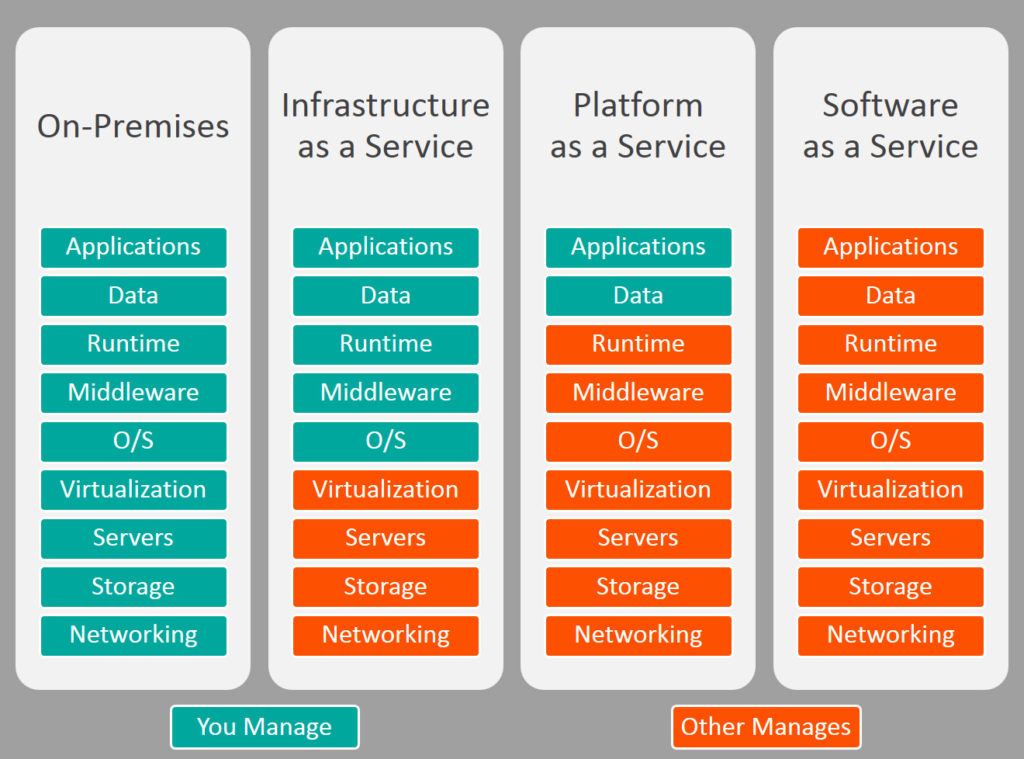
\includegraphics[width=1\textwidth]{imagenes/capitulo1/iaas-paas-saas-comparison.png}
    \caption{Clasificación de cloud computing en base a los recursos que se gestionan.}
	\vspace{0.3cm}
    \footnotesize{Fuente: Stephen Watts, “SaaS vs PaaS vs IaaS: What’s The Difference and How To Choose”, bmc blogs, 2017}    
    \label{comparacion-cloud}
\end{figure}

El concepto de \textit{computación en la nube} es muy amplio, hasta el punto de que podemos afirmar que no existe tal cosa como la computación en la nube. Si le pide a un usuario final que explique qué es la computación en la nube y luego le hace la misma pregunta al administrador del sistema, obtendremos dos descripciones diferentes. En general, hay tres enfoques importantes cuando se trata de computación en la nube dependiendo de los tipos de recursos que se gestionen. En la Fig.\ref{comparacion-cloud} se puede ver esta clasificación tomando como referencia un despliegue tradicional donde se gestionan todos los recursos. Otro punto de vista que lleva a la misma división es, de acuerdo al usuario final de la nube (Fig.\ref{clas-cloud-usuario}):

\begin{itemize}
\item 
\textbf{IaaS (\textit{Infrastructure as a Service})}: Es una infraestructura que se utiliza para proporcionar máquinas virtuales. Va más allá de la virtualización porque la nube agrega escalabilidad y aspectos bajo demanda a la virtualización ofreciendo un control total sobre la infraestructura disponiendo de mecanismos de procesamiento, almacenamiento, red y otros recursos computacionales. Ejemplos de este tipo de arquitectura son: Amazon Web Services, Rackspace Cloud Servers o Mirantis Cloud Platform .
\end{itemize}


\begin{itemize}
\item 
\textbf{PaaS (\textit{Platform as a Service})}: El proveedor suministra la red, los servidores, el almacenamiento, el sistema operativo y el middleware para alojar una aplicación, como casos de uso tenemos: Google App Engine, Windows Azure, OpenShift o Heroku
\end{itemize}

\begin{itemize}
\item \textbf{SaaS (\textit{Software as a Service})}: El proveedor da acceso a una aplicación alojada en la nube como ocurre por ejemplo en Google Apps o Dropbox.
\end{itemize}

\jorge{Pon la fuente en la figura \ref{clas-cloud-usuario} (o dibújala tú, como veas).}

\begin{figure}[!ht]  \centering
    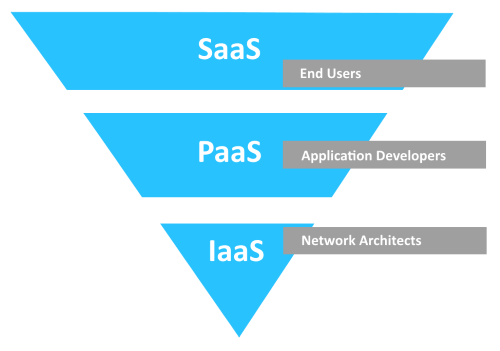
\includegraphics[width=1\textwidth]{imagenes/capitulo1/saas-paas-iaas.png}
    \caption{Clasificación de cloud computing en función del usuario.}
	\vspace{0.3cm}
    \label{clas-cloud-usuario}
\end{figure}

\begin{figure}
    \centering
    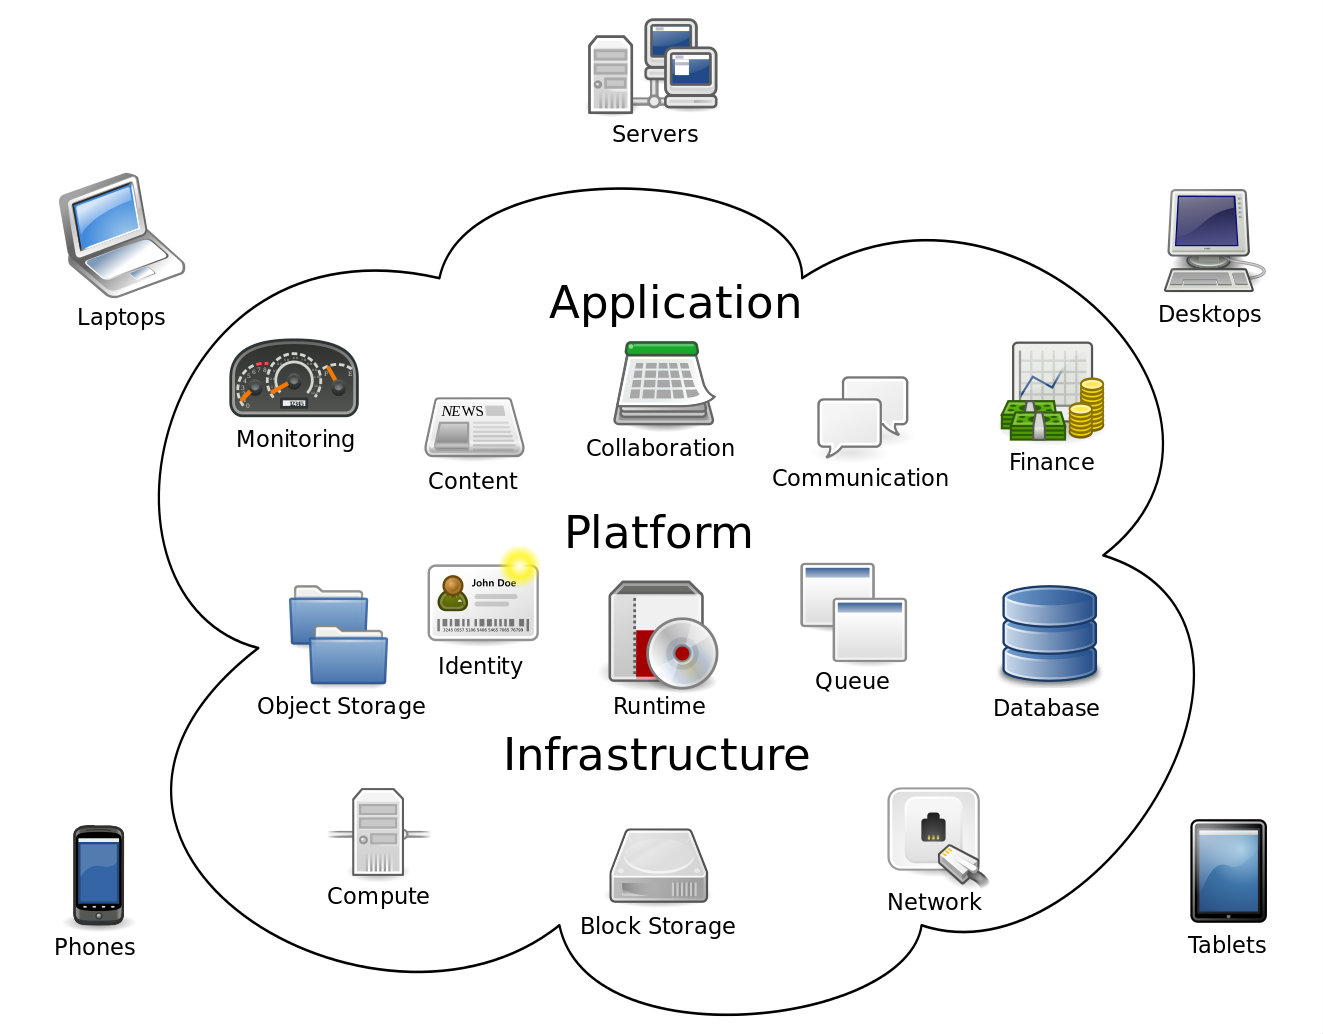
\includegraphics[width=1\textwidth]{imagenes/capitulo1/cloudcomputingDoit.png}
    \caption{Entorno Cloud Computing.}
	\vspace{0.3cm}
    \footnotesize{Fuente:Sam Johnston, "Cloud Computing", licensed underCC BY-SA 3.0 Unported, retrieved from Wikipedia)}
    \label{cloudcomputingDoit}
\end{figure}

En la Fig.\ref{cloudcomputingDoit} podemos ver representado todo lo que realmente podemos hacer en Cloud Computing. Vemos una nube a la que se puede acceder desde teléfonos, portátiles, servidores, escritorios y tabletas, realmente  es accesible desde  cualquier dispositivo. Dentro de la nube tenemos aplicaciones, plataformas e infraestructura. La infraestructura es la nube IaaS. En la nube IaaS, se están proporcionando recursos de cómputo, almacenamiento en bloque y redes. Luego está la plataforma, que es la plataforma como servicio en la nube (PaaS), en la que se proporcionan el almacenamiento de objetos, servicios de identificación, el tiempo de ejecución de los procesos, la cola y la base de datos. Y por último, en la capa más alta, tenemos la nube de aplicaciones que conocemos como nube de software como servicio (SaaS), en la que se están ofreciendo aplicaciones que pueden ser muy diversas, como los ejemplos que aparecen en la figura de monitorización, contenidos específicos, colaboración, comunicación o finanzas.

\subsection{Beneficios del cloud computing}
La computación en la nube presenta diversos beneficios. Hace que las IT sean flexibles para los usuarios así como también para los administradores:


\begin{itemize}
\item Proporciona fácil acceso a los activos de IT esenciales. Esto hace que sea lo más fácil posible para los usuarios emplear estos activos.
\end{itemize}

\begin{itemize}
\item Permite el autodespliegue. Los usuarios ya no necesitan un administrador de IT para implementar un nuevo servidor.
\end{itemize}

\begin{itemize}
\item Proporciona escalabilidad. Cuando se quede sin recursos físicos, es fácil agregar nuevos recursos.
\end{itemize}

\subsection{Modelo de Servicio IaaS}
Como hemos comentado ya, OpenStack se basa inicialmente en un modelo IaaS. Las nubes IaaS se pueden ofrecer de diferentes maneras, utilizando diferentes modelos de servicio:


\begin{itemize}
\item \textbf{Nube privada (\textit{Private Cloud})}. Una empresa crea una infraestructura IaaS que es solo para uso privado.
\end{itemize}

\begin{itemize}
\item \textbf{Nube pública (\textit{Public Cloud})}. La capacidad de la nube se ofrece como un servicio básico, como es el caso de la telefonía que ofrece un proveedor de telecomunicaciones. Los clientes contratan una parte de la infraestructura de la nube pública.
\end{itemize}

\begin{itemize}
\item \textbf{Nube híbrida (\textit{Hybrid Cloud})}. Este tipo de servicio IaaS es un modelo en el que una sesión en la nube consta de componentes de IaaS privados y públicos.
\end{itemize}

\subsection{Funcionamiento del modelo IaaS}
El funcionamiento de la computación IaaS es el siguiente: un usuario final accede al portal de la nube para derivar una máquina virtual. Mientras se prepara la instancia, el usuario final toma decisiones sobre redes, almacenamiento y seguridad. El almacenamiento persistente es opcional. Al final de la vida útil de la VM, esta desaparecerá. 

La nube IaaS proporciona una plataforma flexible para ejecutar contenedores, así como máquinas virtuales, de una manera flexible:

\begin{itemize}
\item La nube IaaS ofrece un portal de autoservicio.
\item También se proporciona almacenamiento escalable y conexión en red.
\end{itemize}

La computación en la nube IaaS funciona mejor para entornos que necesitan soluciones de IT flexibles. Si no necesitamos escalabilidad y autoservicio, quizás sea mejor optar por otro tipo de virtualización.

\section{NFV}

OpenStack Foundation describe NFV (\textit{Network Function Virtualization}) simplemente como una nueva forma de definir, crear y administrar funciones y servicios de red al reemplazar dispositivos físicos dedicados, con software que puede ser automatizado y administrado por OpenStack.

Al igual que las máquinas virtuales tomaron el lugar de muchos servidores dedicados en los centros de datos, NFV simplemente continúa con la mentalidad de reemplazar hardware físico inflexible y patentado por software. Una muestra de ello podemos verla en la Fig.\ref{clasicovsnfv}. 

Es aquí donde entran en juego las funciones de red virtuales (\textit{Virtual Network Function, VNF}). Las VNF son responsables de completar tareas de red específicas, y pueden ser máquinas virtuales, un contenedor, abarcar múltiples contenedores, múltiples máquinas virtuales o servidores bare metal, todo en la parte superior de la infraestructura informática y de red subyacente. 

Algunos ejemplos de VNF son puertas de enlace o \textit{gateways} móviles, \textit{routers}, servicios de red de entrega de contenido, cortafuegos, aceleradores WAN, DNS e incluso funciones básicas de paquete, todas ellas implementadas de manera virtual.


\begin{figure}[!ht]  \centering
    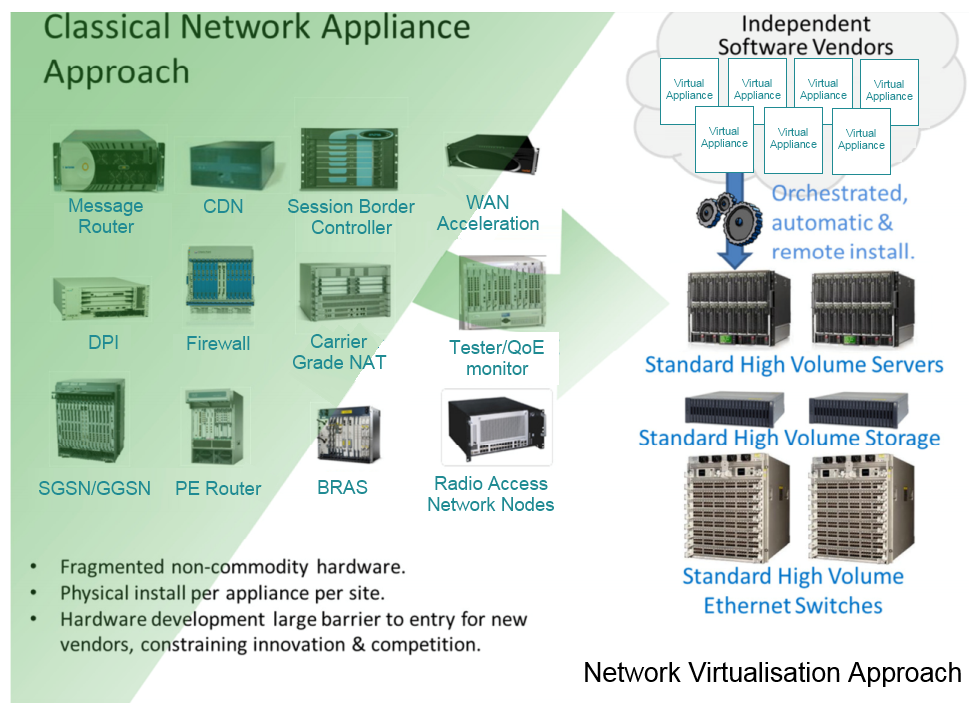
\includegraphics[width=1\textwidth]{imagenes/capitulo1/clasicovsnfv.png}
    \caption{Infraestructura física propietaria vs NFV.}
	\vspace{0.3cm}
    \footnotesize{Fuente: ETSI}
    \label{clasicovsnfv}
\end{figure}

\subsection{Beneficios de NFV}
En general, la mayoría de los beneficios de NFV se centran en agilidad, flexibilidad y simplicidad. Hoy en día, la industria de las telecomunicaciones es más competitiva que nunca y con los márgenes decrecientes, los costos y la demanda de nuevos servicios en aumento, NFV promete ofrecer algunas soluciones viables nuevas. Algunos de los beneficios detallados de NFV son los siguientes:


\begin{itemize}
\item Flexibilidad en la red a través del aprovisionamiento automatizado.
\item Aprovechamiento de la tecnología de código abierto y la innovación.
\item La flexibilidad de los controladores y complementos.
\item Completo acceso y uso de APIs que permiten un desarrollo más rápido.
\item El uso de hardware COTS (\textit{Commercial Off-The-Shelf}) frente a los dispositivos patentados.
\item Eficiencia operativa de una mejor orquestación en centros de datos, regiones y empresas.
\item Amplia gama disponible de documentación.
\end{itemize}

Los beneficios de NFV en OpenStack (frente a otras plataformas) aumentan la eficiencia y reducen los requisitos de Capex y Opex (inversión y gasto), potencia y espacio \cite{silverman_what_2018}.

\subsection{Diferencias entre NFV y SDN}
Aunque NFV y SDN son similares, ambas tienen claras diferencias. Tanto SDN como NFV son una forma de proporcionar funciones de red y automatización de redes heredadas, pero el objetivo de SDN es diferente de NFV. 

SDN consiste en la softwarización de las redes con el fin de simplificarlas, hacerlas más flexibles y reducir costes. Para ello usa un controlador encargado de ejecutar el software que gestiona elementos de red física como \textit{switches}, \textit{firewalls} y \textit{routers}, implementándose en la parte superior de la infraestructura de red física sobre la que se ejecuta la nube. 

NFV consume estas SDN como parte de una solución más grande y luego agrega funcionalidad adicional sobre las SDN. Algunos ejemplos de esto son \textit{firewalls} virtuales, filtros de contenido, aplicaciones antivirus, balanceadores de carga, \textit{routers}, etc. Estas funciones adicionales se denominan VNF o funciones de red virtuales. Aunque SDN juega un papel importante en el aprovisionamiento de recursos de NFV, la misión de NFV es virtualizar las funciones del nivel de aplicación sobre las de SDN \cite{silverman_difference_2018}.

A pesar de estas diferencias, en OpenStack se suele referenciar a los elementos de conectividad de red creados por \textit{Neutron}, proyecto que veremos en la sección \ref{subsec:Neutron}, como SDN.

\jorge{Yo quizá quitaría esa última frase. No aporta mucho sino que más bien lía. OpenStack usa una red SDN virtualizada (es decir, con switches software en lugar de switches físicos) para la red de interconexión de los nodos de cómputo y demás elementos. Pero eso no tiene nada que ver con que luego se implementen VNFs sobre OpenStack.}

\subsection{ETSI}
En los últimos años, la arquitectura NFV ha crecido más allá de ser simplemente una prueba de concepto para el administrador de infraestructura virtual (\textit{Virtual Infrastructure Manager}, VIM) principal que se utiliza para orquestar herramientas de gestión y orquestación de servicios automatizados para la infraestructura de NFV. Sin embargo, para definir mejor las especificaciones de lo que debería ser una plataforma de NFV, los grupos de expertos de OpenStack y los líderes de la industria de las telecomunicaciones han creado un gabinete específico alrededor de las NFV en Telecomunicaciones.

Fundada en 2012 por siete de los mayores operadores de redes de telecomunicaciones, la ETSI (European Telecommunication Standars Institute) creó el Grupo de especificación industrial de facto para NFV. Tras 5 años y más de 100 publicaciones después, lo que comenzó como una prueba de concepto ahora se ha convertido en la base para el estudio de mecanismos de de interoperabilidad. Los resultados de estas pruebas producen estándares para las organizaciones miembro y la industria europea de TIC en general.\cite{noauthor_etsi_nodate}

La ETSI actualmente está trabajando en la definición de la arquitectura y los requisitos para las VNF con el fin de:

\begin{itemize}
\item Maximizar la estabilidad y garantizar la confiabilidad del servicio.
\item Integración fluida con plataformas existentes y servicios heredados EMS, NMS, OSS, BSS y de orquestación de red.
\item Desarrollo de soluciones altamente efectivas y portátiles que tengan una amplia aplicación para proveedores de servicios.
\item Maximizar la eficiencia en la migración a nuevas plataformas virtualizadas.
\item Simplificar y optimizar las operaciones de telecomunicaciones.
\end{itemize}

\begin{figure}
    \centering
    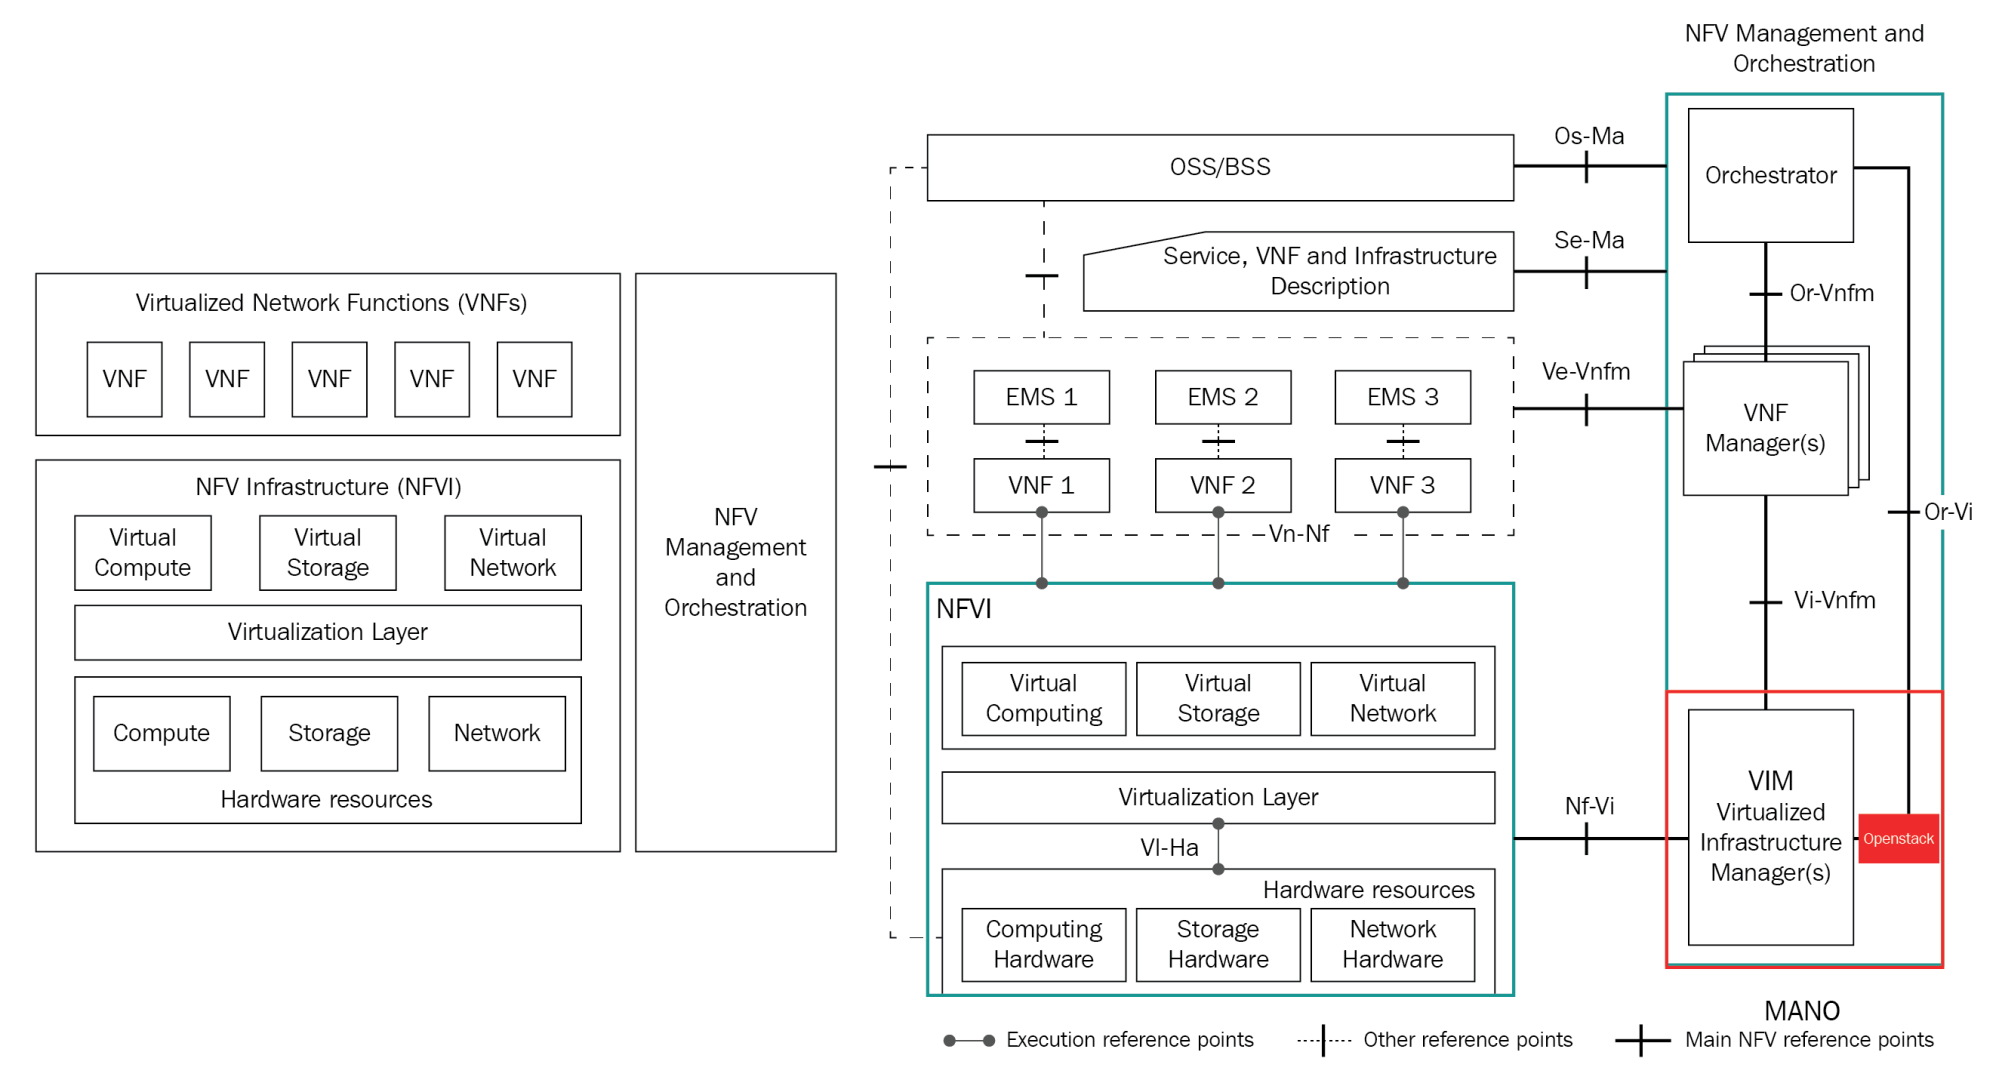
\includegraphics[width=1\textwidth]{imagenes/capitulo1/NFV_arquitectura.png}
    \caption{ETSI MANO Architectural Framework. Arquitectura para  NFV.}
	\vspace{0.3cm}
    \footnotesize{Fuente: ETSI NFV architecture}
    \label{arquitectura-NFV}
\end{figure}

\subsection{El rol de Openstack en NFV}
En la imagen de la Fig.\ref{arquitectura-NFV} podemos ver la base para construir todos los sistemas NFV. En la parte de la izquierda se muestra la arquitectura general de NFV y los principales componentes mientras que en la derecha tenemos como esos componentes funcionan conjuntamente.

El rol de OpenStack es del VIM. El VIM orquesta el hardware contenido en el cuadro de infraestructura NFVI (NFV Infrastructure) para ejecutar las VNFs.


